\newpage
\section{Implementations}
\subsection{NTL et FLINT}
We first sought to measure the performance given to us by existing software. Thus, we can then try to improve them or at least get closer to their performance.
Our work concentrates on polynomials. As such the classes used in both the FLINT and the NTL library relate to polynomial operations.
\subsubsection{NTL}

We started out by familiarizing ourselves with C++ and and the NTL library.
After implementing different time measurement functions we found these results for different degrees of polynomials on different operations but with a fixed set of bits at 60 (the number will be on 60 bits) and generating a polynome with FFTInit (which is way faster then GenPrime\_long which generates a polynome by using different FFT techniques).
The commands we used looked like this 
\begin{lstlisting}[language=bash]
./graph <choice of implementation> <choice of operation> 
<degree of polynomial> <number of bits> <file to save results (TODO)>
<choice of implementation> can either be
        - 0 : using a FFT generated polynomial
        - 1 : using a bits generated polynomial
<choice of operation> can be:
        - 0 : addition
        - 1 : multiplication
        - 2 : GCD
        - 3 : division  (divided by 2 by default (TODO))
        - 4 : XGCD 
For example, you could try ./ntl 0 1 1000 60
Polynome generated with FFT
./ntl 0 1 10000000 60
\end{lstlisting}

(A CHANGER : serait-il possible d'avoir les informations sur l'ordinateur que vous avez utilise ? (notamment avec la commande lshw ou uname -a par exemple))
Also, these operations were run on a macOS Monterey with a Apple M1 chip and 16GB of RAM. The computer was plugged in during these computations.
Running the command 
\begin{lstlisting}[language=bash]
uname -a 
\end{lstlisting}
gives us:
\begin{lstlisting}[language=bash]
Darwin elinas-macbook-air.home 21.6.0 Darwin Kernel Version 21.6.0: Sat Jun 18 17:05:47 PDT 2022; root:xnu-8020.140.41~1/RELEASE_ARM64_T8101 arm64
\end{lstlisting}

We get these results for polynomial multiplication and division:

\begin{figure}[H]
    \centering
    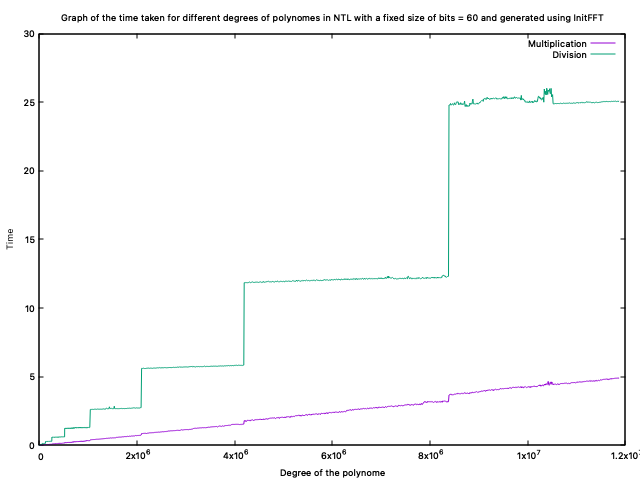
\includegraphics[width=0.85\textwidth]{figures/ntl_mult_div.png}
    \label{fig2}
    \caption{Multiplication and division in NTL}
\end{figure}
NTL uses the Karatsuba algorithm for small polynomials and the Fast Fourier Transform (FFT) or NTT for larger polynomials. The complexity for polynomial multiplication using these algorithms is:
\begin{itemize}
    \item Karatsuba: $O(n^{1.585})$, where $n$ is the degree of the polynomials
    \item FFT-based algorithms: $O(n\log(n))$
    \item NTT-based algorithms: $O(n\log(n))$
\end{itemize}
For the polynomial division, NTL uses the classical polynomial division algorithm, which has a complexity of:
\begin{itemize}
    \item Classical division: $O(n^2)$, where $n$ is the degree of the divisor polynomial
\end{itemize}

For the GCD and the XGCD we get the graphs :
\begin{figure}[H]
    \centering
    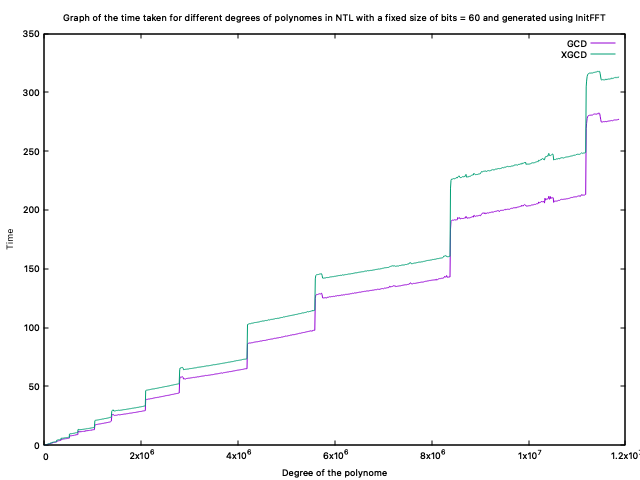
\includegraphics[width=0.85\textwidth]{figures/ntl_gcd_xgcd.png}
    \label{fig2}
    \caption{GCD and XGCD (a*u + b*v = p format) in NTL}
\end{figure}

For polynomial GCD and XGCD computations, NTL uses the Euclidean algorithm. The complexity of this algorithm is:
\begin{itemize}
    \item Euclidean algorithm: $O(n^2)$, where $n$ is the degree of the input polynomials
\end{itemize}
\subsubsection{FLINT}

Then we wanted to measure the results for another popular library for number theory FLINT. 
To get better and more representative results, we separated the XGCD and the GCD from the multiplication and the division as those operations were closer to each other in terms of the time they were taking.

For the multiplication and the division we get:
\begin{figure}[H]
    \centering
    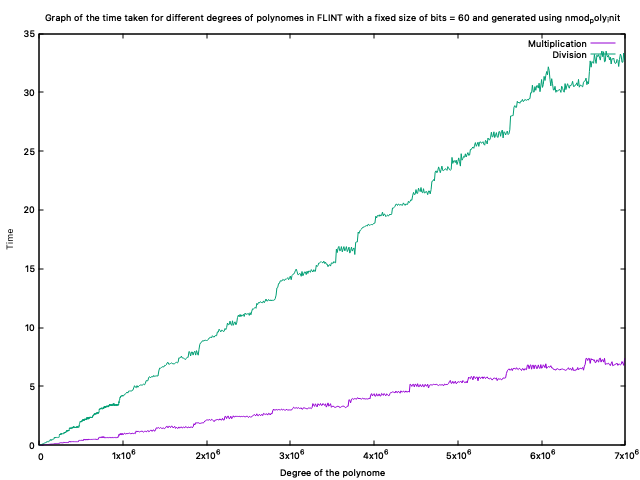
\includegraphics[width=0.85\textwidth]{figures/flint_mult_div.png}
    \label{fig2}
    \caption{Multiplication and division in FLINT}
\end{figure}
For polynomial multiplication, FLINT uses a combination of algorithms, such as the schoolbook method for small polynomials, Karatsuba's algorithm for medium-sized polynomials, and the Fast Fourier Transform (FFT) or NTT for large polynomials. The complexity of these algorithms is:
\begin{itemize}
    \item Schoolbook method: $O(n^2)$, where $n$ is the degree of the input polynomials
    \item Karatsuba's algorithm: $O(n^{1.585})$, where $n$ is the degree of the input polynomials
    \item FFT-based algorithms: $O(n \log(n))$, where $n$ is the degree of the input polynomials
    \item NTT-based algorithms: $O(n \log(n))$, where $n$ is the degree of the input polynomials
\end{itemize}
For polynomial division, FLINT uses the classical polynomial division algorithm, which has a complexity of:
\begin{itemize}
    \item Classical division: $O(n^2)$, where $n$ is the degree of the divisor polynomial
\end{itemize}

And for the GCD and the XGCD we get the graphs :
\begin{figure}[H]
    \centering
    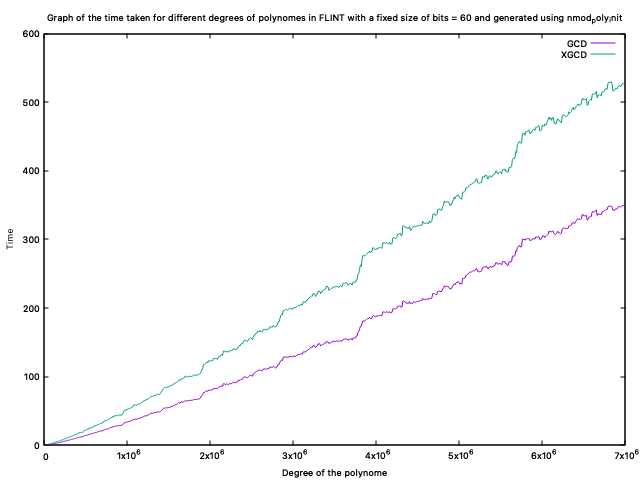
\includegraphics[width=0.85\textwidth]{figures/flint_gcd_xgcd.png}
    \label{fig2}
    \caption{GCD and XGCD (a*u + b*v = p format) in FLINT}
\end{figure}
For polynomial GCD and XGCD computations, FLINT uses various algorithms depending on the input size, such as the Euclidean algorithm for small input polynomials and the half-GCD algorithm for larger input polynomials. The complexity of these algorithms is:
\begin{itemize}
    \item Euclidean algorithm: $O(n^2)$, where $n$ is the degree of the input polynomials
    \item Half-GCD algorithm: $O(n \log^2(n))$, where $n$ is the degree of the input polynomials
\end{itemize}

\qquad As such those are the results we want to approximate using our algorithm.